\documentclass[sigconf]{acmart}
\usepackage{booktabs}
\usepackage{svg}
\usepackage{algorithm}
\usepackage[noend]{algpseudocode}

%% \BibTeX command to typeset BibTeX logo in the docs
\AtBeginDocument{%
  \providecommand\BibTeX{{%
    \normalfont B\kern-0.5em{\scshape i\kern-0.25em b}\kern-0.8em\TeX}}}

%% These commands are for a PROCEEDINGS abstract or paper.
\settopmatter{printacmref=false} % Removes citation information below abstract
\renewcommand\footnotetextcopyrightpermission[1]{} % removes footnote with conference information in 

\acmConference[AEPRO 2023]{AEPRO 2023: Algorithm Engineering Projects}{March 1}{Jena, Germany}

% convert text to title case
% http://individed.com/code/to-title-case/

% that helps you to formulate your sentences
% https://www.deepl.com/translator

\begin{document}


%%
%% The "title" command has an optional parameter,
%% allowing the author to define a "short title" to be used in page headers.
\title[Generating 2D Datsets with similar statistical properties]{Generating 2D Datsets with similar statistical properties\\\large Algorithm Engineering 2023 Project Paper}

%%
%% The "author" command and its associated commands are used to define
%% the authors and their affiliations.

\author{Veit Hucke}
\affiliation{%
  \institution{Friedrich Schiller University Jena}
  \country{Germany}}
\email{veit.hucke@uni-jena.de}

\author{Marius Wank}
\affiliation{%
  \institution{Friedrich Schiller University Jena}
  \country{Germany}}
\email{marius.wank@uni-jena.de}

%% The abstract is a short summary of the work to be presented in the article.
%% Topic and background: What topic does the paper deal with? What is the point of departure for your research? Why are you studying this now?
%% Focus: What is your research question? What are you studying precisely?
%% Method: What did you do?
%% Key findings: What did you discover?
%% Conclusions or implications: What do these findings mean? What broader issues do they speak to?
\begin{abstract}

%% Here we write the abstract
Teaching how to interpret statistical properties of data is an important task. Making assumptions about the data we handle purely based on their statistical properties 
is a pitfall that can easily be avoided by highlighting the importance of data visualization. In this paper we present an algorithm that tackles that task while also 
accommodating  the need for hardware-optimized algorithms to handle today’s  large amounts of data. Our algorithm improves on the code created by Justin Matejka and George 
Fitzmaurice by implementing it in C++ and introducing parallelism as well as vectorization to it. The idea is to generate a scatter plot with a target shape while maintaining 
identical statistical properties to an input dataset through simulated annealing. Our experiments show that even a naive conversion from Python to C++ can drastically
improve performance and allows access to several tools that can widen the gap even further. Using these tools, we successfully improved the runtime of the code by up to 105x.
We conclude that, even though the implementation is harder, utilizing these tools is necessary to handle big data in reasonable amounts of time.  

\end{abstract}

%%
%% Keywords. The author(s) should pick words that accurately describe
%% the work being presented. Separate the keywords with commas.
\keywords{C++, parallelism, vectorization, statistics, data visualization}

%%
%% This command processes the author and affiliation and title
%% information and builds the first part of the formatted document.
\maketitle

\let\thefootnote\relax\footnotetext{AEPRO 2023, March 1, Jena, Germany. Copyright \copyright 2023 for this paper by its authors. Use permitted under Creative Commons License Attribution 4.0 International (CC BY 4.0).}

\section{Introduction}

\begin{figure}[htbp]
  \centering
  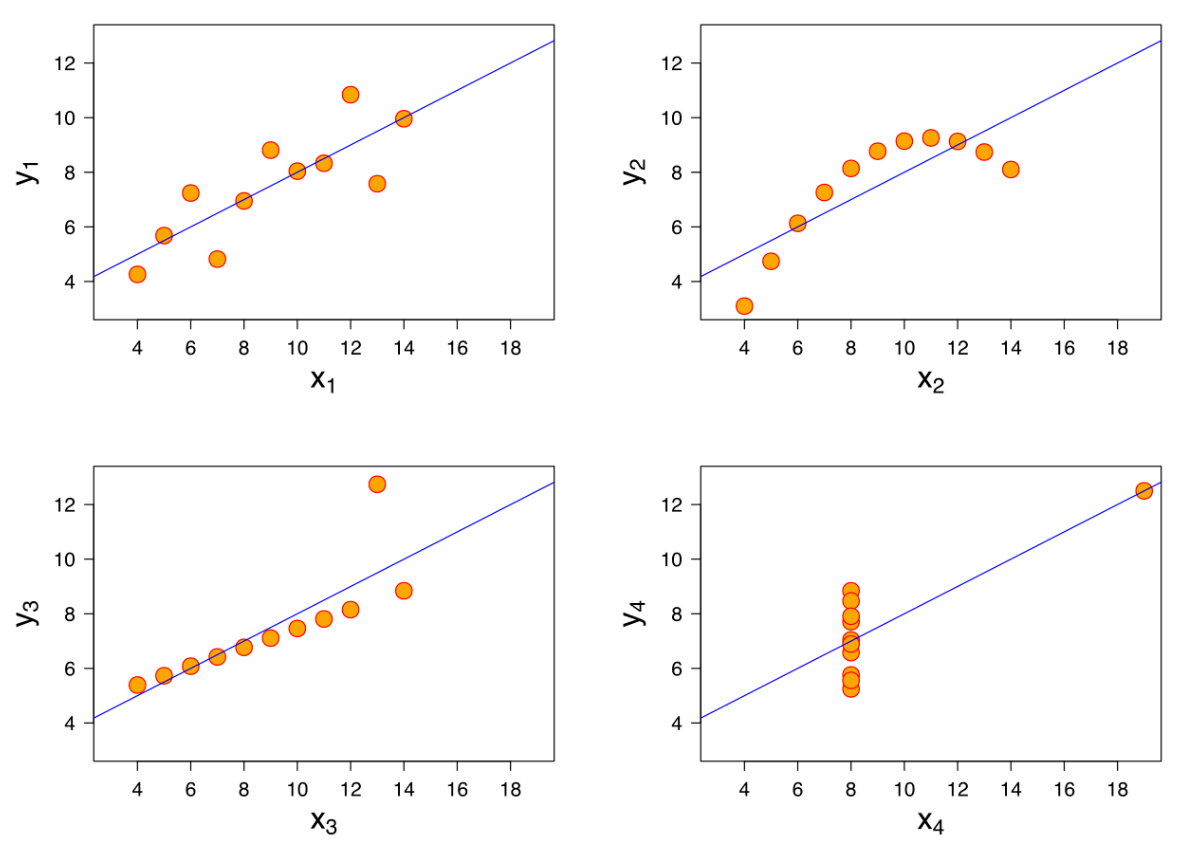
\includegraphics[width=\linewidth]{./graphics/Anscombe.PNG}
  \caption{Anscombe's quartet. Each dataset contains 11 datapoints and has a similar mean of x and y (exact), sample variance of x and y (exact), correlation between x and y (to 2 decimal places), linear regression line (to 3 decimal places for a and to 2 decimal places for c) and coefficient of 
  determination of the linear regression line (to 2 decimal places)\cite{doi:10.1080/00031305.1973.10478966}.}
  \label{fig:integer:Anscombe}
\end{figure}  

\subsection{Background}
%% Write about educational purpose (history; Anscombe's quartet) -> showing the importance of visualizing data, maybe some inspiration from original paper (from autodesk)
According to Francis John Anscombe graphs are an important tool to gain a better understanding during statistical analysis\cite{doi:10.1080/00031305.1973.10478966}. He argues that by only looking at the statistical properties
of data and not visualizing it we will only get a limited understanding of that data. To support his claim he created Anscombe's quartet, a visualization of four statistically  nearly identical datasets (see Figure~\ref*{fig:integer:Anscombe}). 
The graph shows that, even though similar in properties, the datasets are vastly different. To further underline his point, we wanted to expand upon his idea and improve an algorithm that could generate any given target shape from a given dataset 
while maintaining statistical properties similar to the original. We decided to use the work of Matejka and Fitzmaurice\cite{10.1145/3025453.3025912} as our starting point.\newline\newline According to Moore's Law from 1965 the number of
transistors on a computer chip (and therefore its power) will double every two years\cite{moore1965cramming}. Nowadays we know that this law does not hold anymore as we approach physical limitations. With this in mind we also wanted to design our
algorithm in a way that it utilizes modern techniques to improve runtime, meaning a hardware-specific implementation.


\subsection{Related Work}
%% Write about the paper from autodesk; what and how they did it

As mentioned above, the algorithm by Matejka and Fitzmaurice\cite{10.1145/3025453.3025912} generates any given target shape from a given dataset while maintaining statistical properties similar to the original. The similarity is limited
to 2 decimal places. Their idea was that even though creating a fully new dataset with similar properties is difficult, iteratively changing an existing one marginally to conserve the properties is easy. This was achieved by performing a small, biased 
perturbation on the dataset every iteration, where a translocation of a point is only accepted when it moves towards the target shape. To prevent getting stuck on local optima, a small chance that decreases every iteration is given to accept perturbations 
that did not move a point towards the target shape. After each iteration a check is done to see if the change of statistical properties was within a given threshold. An example on how this process looks like can be found in Figure~\ref*{fig:integer:Autodesk_Example}.\newpage The algorithm
accepting non-optimal solutions is called simulated annealing and was first introduced in 1995 by Kirpatrick et al.\cite{kirkpatrick1995simulated}. It uses the function \(e^{-\frac{\Delta E}{kT}}\) as the probability to accept worse
perturbations, where \(\Delta E\) denotes the difference between the error functions of the current and previous step (in the case of Matejka and Fitzmaurice the distance to the closest point of the target shape), \(k\) the Boltzmann constant and \(T\)
the temperature which is decreased every step to shrink the probability.\newline\newline While this method proves to be successful, the performance leaves a lot of room for improvement. In the paper by Matejka and Fitzmaurice Python is used for the implementation
causing the program to run for several minutes before finishing. Our implementation vastly improves upon that by using C++ as the programming language of choice.\newline\newline Since Matejka and Fitzmaurice covered different generalized methods for creating datasets with
similar statistics and dissimilar graphics we will not present them here to avoid repetition. We do however recommend them for a more in-depth understanding of the subject. These works include the publications by Chatterjee and Firat\cite{10.2307/27643902} as well as 
Govindaraju and Haslett\cite{https://doi.org/10.1111/j.1467-842X.2009.00560.x}. 


\begin{figure}[htbp]
  \centering
  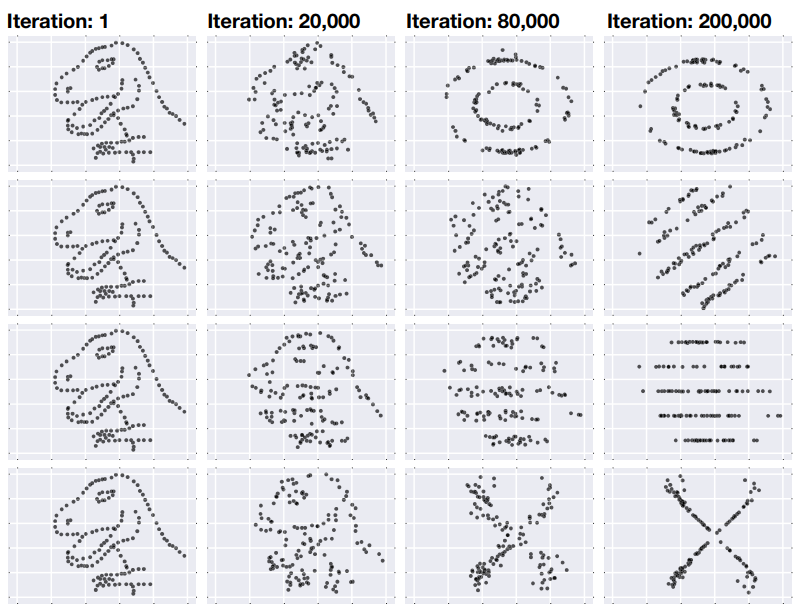
\includegraphics[width=\linewidth]{./graphics/Autodesk_Example.PNG}
  \caption{Example of the simulated annealing process by Matejka and Fitzmaurice. Each dataset has the same summary statistics to two decimal places:
  (\(\bar{x}\)=54.26, \(\bar{y}\) = 47.83, sdx =16.76, sdy = 26.93, Pearson’s r = -0.06). The image and description were taken directly from the original paper\cite{10.1145/3025453.3025912}.}
  \label{fig:integer:Autodesk_Example}
\end{figure}
\newpage

\subsection{Our Contributions}
%% Mention that Moore's law doesn't apply anymore; Parallelsim and vectorization are getting more important
The main goal of this project is to develop an application based on the work of Matejka and Fitzmaurice but with a stronger focus on performance and efficiency. We therefore chose the C++ programming language as a foundation, which is already the biggest difference to the original work.\newline
Besides being inherently more performant than Python, it also allows to have significantly more control over the computer, making it possible to utilize its resources more efficiently. Which further specific improvements and techniques have been implemented will be described in detail in section \ref{sub:sec:improvements}.

\subsection{Outline}
%% Describe what is covered in the upcoming sections (I guess; no idea what else is meant)
In section \ref{algorithm} we are going to talk about the exact implementation of our algorithm. This includes specifics about how input and output data is processed as well as the C++ specific tools used to fabricate a hardware-optimized
version of the simulated annealing approach.\newline\newline In section \ref{experiments} we share the results of our work and the setup that was used to compare our implementation with the one by Matejka and Fitzmaurice.\newline\newline In section \ref{conclusion}
we first discuss our implementation based on efficiency and portability. We also present ideas that can be used to improve our work in the future. In the end we judge if we achieved the goals of this study sufficiently. 


%% EXAMPLE OF FIGURES
%% In Figure~\ref{fig:integer:sets} we convert the mock labels to sorted integer sets.
%% \begin{figure}[htbp]
%% \centering
%% \includegraphics[width=\linewidth]{./graphics/integer_sets.pdf}
%% \caption{Conversion of mock camera labels to sorted integer sets. 
%% We map each unique token (key) in camera labels to a unique value. 
%% Based on these key-value-mappings, we convert camera labels to sorted integer sets.
%% A camera can have different names in different countries. Therefore, repeating IDs reference the same cameras (see, for example, ID=3).} 
%% \label{fig:integer:sets}
%% \end{figure}

%% EXAMPLE OF LISTS

%% \begin{itemize}
%% \item Reading many small files concurrently, with multiple threads (compared to a single thread), takes advantage of the internal parallelism of SSDs and thus leads to higher throughput \cite{Zhuang2016}.
  
%% \item C-string manipulation functions are often significantly faster than their C++ pendants. For example, locating substrings with \texttt{strstr} is around five times faster than using the C++ \texttt{std::string} function \texttt{find}.
  
%% \item Hardcoding regular expressions with \emph{while, for, switch} or \emph{if-else} statements results in faster execution times than using standard RegEx libraries, where regular expressions are compiled at runtime into state machines.
  
%% \item Changing strings in place, instead of treating them as immutable objects, eliminates allocation and copying overhead.
  
%% \end{itemize}

%% EXAMPLE OF TABLE

%% Table~\ref{tab:results} shows the running times of the resolution step of the five best placed teams.

%% \begin{table}[htbp]
%% \caption{Comparison of the F-measure and the running times of the resolution step of the five best placed teams. The input data for the resolution step consisted of 29{,}787 in JSON formatted e-commerce websites. Measurements were taken on a
%% laptop running Ubuntu 19.04 with 16 GB of RAM and two Intel Core i5-4310U CPUs. The underlying SSD was a 500\,GB 860 EVO mSATA. We cleared the page cache, dentries, and inodes before each run to avoid reading the input data from RAM instead of the SSD.}
%% \label{tab:results}
%% \resizebox{\columnwidth}{!}{
%% \begin{tabular}{lcrr}
%% \toprule
%% Team& Language & F-measure & Running time (s)\\
%% \midrule
%% PictureMe (\textbf{this paper}) &C++& 0.99 & \textbf{0.61}\\
%% DBGroup@UniMoRe &Python& 0.99 & 10.65\\
%% DBGroup@SUSTech &C++& 0.99 & 22.13\\
%% eats\_shoots\_and\_leaves &Python& 0.99 & 28.66\\
%% DBTHU &Python& 0.99& 63.21\\
%% \bottomrule
%% \end{tabular}
%% }
%% \end{table}



\section{The Algorithm} \label{algorithm}

\subsection{Handling of input data}
\label{sub:sec:input}
The basic approach we follow in our implementation is similar to the approach by Matejka and Fitzmaurice, but small adjustments have been made. In our implementation we only use the Datasaurus dataset as the input for demonstration
purposes so the user only has to enter the preferred target shape as well as a path where the preferences.json is located. We use the preferences.json as a way to reduce the number of parameters the user has to enter in the command line. We
did not implement support for all possible target shapes from the original paper as time was a limiting factor. After starting the program, the correctness of the input is checked and a dataframe is created from the Datasuarus dataset. After that the
statistical properties of the input dataset are calculated and perturbations on the dataset are run through simulated annealing as long as defined by the user. 

\subsection{Simulated annealing}
\label{sub:sec:annealing}
The algorithm that ensures both a perturbation towars a desired target shape and the conservation of the statistical properties of the original data is based on simulated annealing. There are other possibilities to achieve this goal, such as using genetic algorithms, but we chose to stick to the implementation of the original authors\cite{10.1145/3025453.3025912} because of its simplicity.

\begin{algorithm}[H]
\caption{}
\begin{algorithmic}[1]
	\State $current\_df\gets initial\_df$
	\State $new\_df\gets initial\_df$
	\For{$\text{n iterations}$}
		\State $new\_df\gets Perturb(current\_df,temp)$
		\If{$is\_error\_okay(new\_df,current\_df)$}
			\State $current\_df\gets new\_df$
		\EndIf
	\EndFor
	
\Function{$Perturb$}{$df,temp$}:
	\State $pos\gets Random()$
	\State $orig\_point\gets df[pos]$
	\Loop
		\State $new\_point\gets MoveRandom(orig\_point)$
		\If{$Dist(new\_point)<Dist(orig\_point)$\newline
		\textbf{or} $temp>Random()$}
			\State $new\_df\gets df$
			\State $new\_df[pos]\gets new\_point$
		\EndIf
	\EndLoop
	\Return{$new\_df$}
\EndFunction
\end{algorithmic}
\end{algorithm}

In general, a \textit{perturb\_once()} function is called which accepts a DataFrame, containing the x- and y-coordinates of all points specified in the imported file. A random (x, y) pair from the input DataFrame is drawn and perturbed slightly. The value by which the original pair is modified is normal distributed which is itself modified by a factor \textit{shake} specified by the user. The euclidean distance of both the original pair (x, y), as well as the modified pair (x\_new, y\_new) is calculated and compared. Now there are multiple condition that can be met in order to assert a successful perturbation of the data:\newline
The most intuitive condition is that the distance of the modified point to the target shape is smaller than that of the original point. Alternatively, a worse state of the system can also be accepted, based on a temperature randomly drawn from the distribution unif[0.0, 1.0). This is part of the actual simulated annealing and prevents the system to eventually get stuck in a local optimum. As a cooling schedule, we adapted the smoothed monotonic function proposed by Matejka and Fitzmaurice to preserve comparability. The schedule starts at a temparature of 0.4 and terminates at a temperature of 0.01 per default, but these values may also be altered by the user. Finally, if the new distance is smaller than a lower bound \textit{allowed\_distance} defined by the user, the new state is accepted as well. This is because we consider a pair (x, y) being optimal and in its final position as soon as this threshold is reached.\newline
This perturbation-comparison mechanism is repeated as long as none of these conditions are met. However, if one condition eventually becomes true, a copy of the initial DataFrame is made, the new points are overwritten and the copy is returned by the function.\newline
The \textit{perturb\_once()} function itself is called for multiple iterations, where after each iteration a function \textit{is\_error\_okay()} is called that ensures the conservation of the statistical properties. As in the original work from Matejka and Fitzmaurice, we consider the properties conserved if they are equal to two decimal points. If this is the case, the initial DataFrame is overwritten with the slightly modified one, the data of the new DataFrame is written to a buffer and the next iteration of \textit{perturb\_once()} is invoked. Otherwise, the initial DataFrame will not be overwritten and it goes into the next iteration of modification as well.

\subsubsection{Improvements}
\label{sub:sec:improvements}
As mentioned above, using the C++ programming language was not only the first major performance improvement that has been achieved, it also allowed having more control over the computer.\newline
\textit{Vectorization}. Keeping in mind that the data the algorithm works on is stored in large vectors, using vectorization is an obvious technique to implement. The statistical properties have to be calculated in every iteration to ensure that they do not change due to the perturbation of single points, so applying the same operations on huge chunks of data implies a significantly more efficient usage of the computers resources. The vectorization is achieved by guiding the compiler using the \textit{omp simd} pragma. Furthermore, loops in the statistical methods are additionally accelerated by using the \textit{reduction} clause as the body of the loops only contain simple summations. Finally, the used vectors are 64 byte aligned, supporting the compiler in vectorizing the code and resulting in a faster access and more efficient usage of the bandwidth between main memeory and the CPU.\newline
\textit{Data handling}. To further improve the internal processing of the data, we decided to keep the coordinates in separate x- and y-vectors that are part of a custom DataFrame struct. As the statistical properties are calculated independently for these x- and y-coordinates, the usage of a Structure of Arrays allows a strided 1 memory access, efficiently making use of the 64 byte of a cache line.\newline
We also cosidered a more efficient way to output the data again: Compared to the original script, we did not save multiple .csv files during the iterations. Our algorithm opens an output file once and, everytime an acceptable change in the coordinates happens, the update is saved in a buffer, which is finally written to the file once after all iterations finished.\newline
\textit{RNG}. The standard library of C++ natively supports the generation of random numbers, however, considering performance, the built-in algorithms were still a major bottleneck as they have to be called in every iteration for multiple times. Our approach to improve this hotspot was to implement custom random number generators based on the xoroshiro128+ algorithm\cite{blackman2021scrambled} and the Box-Muller transform to attain uniform and normal distributed numbers respectively.\newline
\textit{Distances}. The original implementation of the algorithm that finds the minimal distance between a point (x, y) and its closest line segment was not working properly for some shapes, such as the \textit{Star}. Due to this circumastance, a new algorithm has been implemented that is based on extending the line segment and projecting the point (x, y) onto it. On the one hand, this algorithm resolved the issue with not finding a fitting optimum for some target shapes. On the other hand, as a positive side effect, the performance was slightly increased as well due to less if...else statements.

\subsection{Processing of output data}
\label{sub:sec:output}
To create the visualization of our output data we decided to stick to Python as it offers the easiest way for creating videos from multiple scatter plots via the libraries matplotlib. First we read the data from the output .csv file using the pandas library to create an iterable dataframe. 
We then simply iterate over the unique frames saved in the .csv, create a dataframe for the x- and y-coordinates corresponding to the current frame and create a scatter plot from these using the matplotlib library.\newpage
Each scatter plot is saved to a list which is used afterwards to create an animation
using the animation class of matplotlib. As a result, we get a .gif file in witch we can see the time evolution of the scatter plot. 

\section{Experiments} \label{experiments}
Table~\ref*{tab:results} shows the comparison between our code and the implementation by Matejka and Fitzmaurice for different target shapes. Our implementation achieves a 54x to 105x faster runtime depending on the concrete target shape. Independent of the target shape the
generation of the output .csv file containing the x- and y-coordinates of the frames took about 0.2 seconds. This means that the visualization Python script we used was responsible for about 90 to 95\% of the runtime in every case. 

\begin{table}[htbp]
\caption{Comparison of the running times of the simulated annealing process plus the visualization for different target shapes for 200{,}000 iterations. The input data was always the Datasaurus dataset from the paper by Matejka and Fitzmaurice. Measurements were taken on a desktop computer,
running Windows 10 Educational with 16 GB RAM and one AMD Ryzen 5 2600X CPU. The underlying SSD was a 256 GB 850 Pro SATA III.}
\label{tab:results}
\resizebox{\columnwidth}{!}{
  \begin{tabular}{lcrr}
  \toprule
  Team& Language & Target shape & Running time (s)\\
  \midrule
 Wank and Hucke &C++ & Circle & \textbf{4.16}\\
 Matejka and Fitzmaurice & Python & Circle & 238\\
  \midrule
 Wank and Hucke &C++ & Bullseye & \textbf{4.41}\\
 Matejka and Fitzmaurice &Python & Bullseye & 242\\
  \midrule
  Wank and Hucke &C++ & Dots & \textbf{2.68}\\
 Matejka and Fitzmaurice & Python & Dots & 283\\
  \midrule
  Wank and Hucke &C++ & X & \textbf{2.76}\\
 Matejka and Fitzmaurice & Python & X & 244\\
  \midrule

  \bottomrule
  \end{tabular}
}
\end{table}

\section{Outlook \& Conclusion} \label{conclusion}
Even though our implementation achieves a vastly faster runtime it is far from perfect. A major bottleneck is the visualization which uses Python, further proving our point that Python should not be used for performance focused programming. In the future the visualization could be 
implemented using C++ graphics libraries like OpenGL or SDL. For the purpose of a more dynamic use of this code a future approach could include taking user input directly via a graphical user interface where the users can draw the input and target shape of the dataset by themselves. We experimented with the
SFML library which proved to be a simple and effective tool. The main reason we did not include it in the final release is that portability was an issue since SFML requires the use of a version that matches the used compiler of the user. We did not want to include every possible 
version as we did not have the time to ensure sufficient portability for every OS and compiler. Also, since this work represents a proof-of-concept, the generated data will always be overwritten when running the code again. To make the program viable for applications outside of testing
it would be a nice addition to have it save multiple different runs separately. Another thing to improve is the usage of our random number generator. The seeds we used for testing purposes are hardcoded and could be changed manually, but a more dynamic approach would be favorable. 
Finally, exception handling is a small but important task to ensure smooth usage of the program. This could include checking the contents of the input and output .csv files for correctness. However, we did not implement handling for all possible exceptions at this time as
this was not necessary in the confined testing setup we used.\newline\newline Even though there are many possibilities to improve our code even further, the here presented results achieved the goal to improve the approach by Matejka and Fitzmaurice and enables users to process big data
in reasonable amounts of time, proving the value of hardware-optimized implementations. 
%%
%% The next two lines define the bibliography style to be used, and
%% the bibliography file.
\bibliographystyle{ACM-Reference-Format} %% Set to unsrt if we want the citations to be numbered by order of appearance.
\bibliography{literature}


\end{document}
\endinput